\documentclass[landscape,12pt]{amsart}
\usepackage{geometry}
\usepackage{amsmath}
\usepackage{amssymb}
\usepackage{graphicx}
\usepackage{subfig}
\usepackage[table]{xcolor}
\usepackage{color}
\usepackage{natbib}

\usepackage{blindtext}
\usepackage{tabularx}

\newenvironment{frcseries}{\fontfamily{frc}\selectfont}{}
\newcommand{\textfrc}[1]{{\frcseries#1}}
\newcommand{\mathfrc}[1]{\raisebox{-0.8mm}{\text{\textfrc{\small #1}}}\hspace{0.4mm}}

\geometry{letterpaper}

%\usepackage[T1]{fontenc}

% general commands
\definecolor{lemonchiffon}{rgb}{1, .98, .80}
\definecolor{lightgrass}{rgb}{.89, 1, .87}
\newcommand{\vect}[1]{\boldsymbol{\mathbf{#1}}}
\newcommand{\degree}[1]{${#1}^{\circ}$}
\newcommand{\highlight}{ \rowcolor{lightgrass} }
\newcommand{\script}[1]{\mathcal{#1}}

\newcommand{\eqn}[1]{\begin{align*}
#1
\end{align*}}
\newcommand{\eqnl}[2]{\begin{align} \label{#1}
#2
\end{align}}
\newcommand{\shblock}{\hspace{3mm}}
\newcommand{\hblock}{\hspace{8mm}}
\newcommand{\eqnsep}{\shblock\hblock}

\newcommand{\bl}{\big\{}
\newcommand{\br}{\big\}}
\newcommand{\Bl}{\Big\{}
\newcommand{\Br}{\Big\}}

\newcommand{\argmax}{\operatornamewithlimits{argmax}}

\newcommand{\indicator}{\mathbf{1}}

\newcommand{\mtx}[4]{
\[
#1 = #2
\left[ {\begin{array}{#3}
 #4
 \end{array} } \right]
\]
}

\newcommand{\eqnset}[4]{
\[ #1 = #2 \left\{ \begin{array}{#3}
        #4
\end{array} \right. \] 
}



        
        
        
        \newcommand{\img}[2]{
	\begin{figure}
		\centering
		\includegraphics[width=\textwidth]{#1}
		\caption{#2}
	\end{figure}
}

\newcommand{\imgi}[1]{
	\vspace{10mm}
	\includegraphics[width=\textwidth]{#1}
	\vspace{10mm}
}


% paper specific terms
\newcommand{\vz}{\vect{z}}
\newcommand{\vx}{\vect{x}}
\newcommand{\vy}{\vect{y}}
\newcommand{\vp}{\vect{\pi}}
\newcommand{\vph}{\hat{\vect{\pi}}}
\newcommand{\vpmle}{\hat{\vect{\pi}}_\text{MLE}}



\newcommand{\fab}{f_j}
\newcommand{\llp}{\mathfrc{l}(\vect{\pi})}

\newcommand{\pims}{1-\pi_1,\ldots,\pi_{m-1}}

\newcommand{\hessll}[2]{\sumn \frac{f_{#1}}{(\summ \pi_j f_j)^2 f_{#2}}}
\newcommand{\hessllg}[2]{\sumn \frac{f_{#1}}{(\sumg \pi_j f_j)^2 f_{#2}}}
\newcommand{\hesslld}[2]{\frac{\partial^2 \llpp}{\partial \pi_{#1} \partial \pi_{#2}}}


\newcommand{\sumn}{\sum^n_{i=1}}
\newcommand{\summ}{\sum^m_{j=1}}
\newcommand{\summo}{\sum^{m-1}_{j=1}}
\newcommand{\sumg}{\sum^g_{j=1}}
\newcommand{\sumk}{\sum^m_{k=1}}

\newcommand{\vpg}{\vp^{\prime}}
\newcommand{\vpgh}{\hat{\vp}^{\prime}}
\newcommand{\llpp}{\mathfrc{l}(\vpg)}
\newcommand{\llpph}{\mathfrc{l}(\vpgh)}


%%% TITLE
\title{Metallicity Smoothing}
\author{\today}

%%% BEGIN DOCUMENT
\begin{document}

\maketitle





\begin{figure}
	\begin{center}
		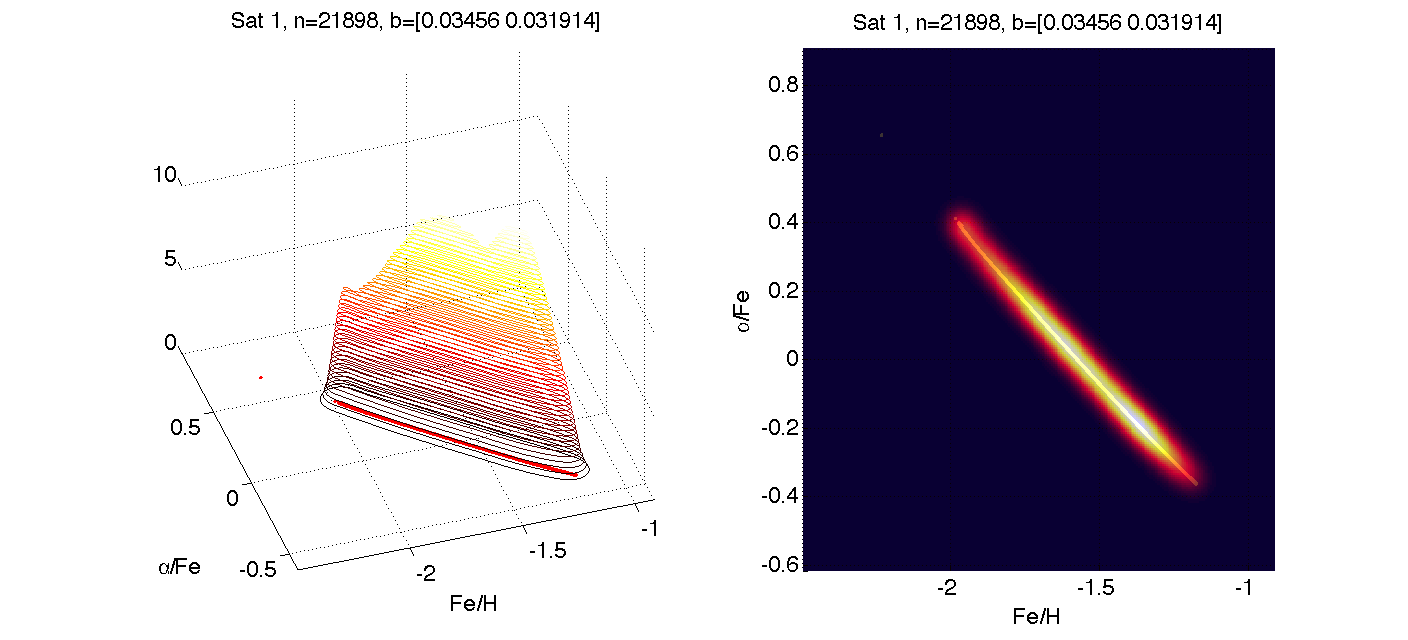
\includegraphics[scale=.5]{smooth1_08.png}
	\end{center}
	\caption{Unweighted kernel density estimate for sat 1 with a manual bandwidth parameter of 0.8 (via t\_star).}
\end{figure}

\begin{figure}
	\begin{center}
		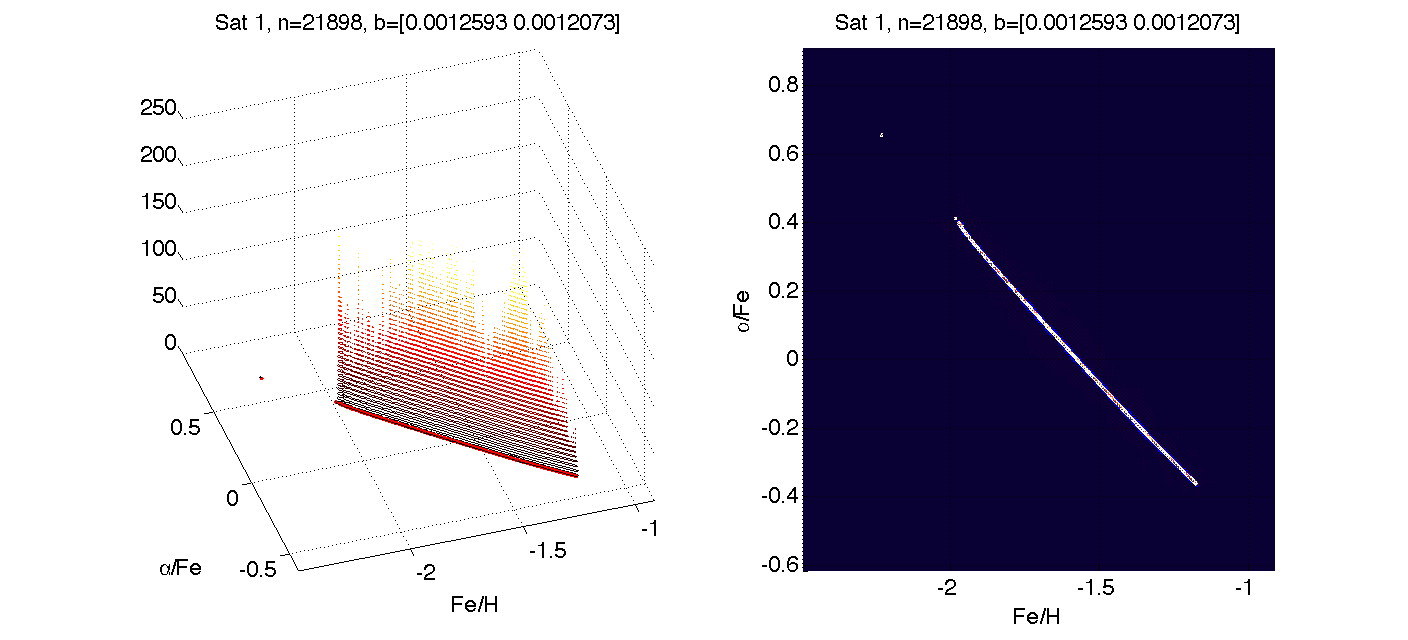
\includegraphics[scale=.5]{smooth1_auto.png}
	\end{center}
	\caption{Unweighted kernel density estimate for sat 1 with an automatic bandwidth.}
\end{figure}

\begin{figure}
	\begin{center}
		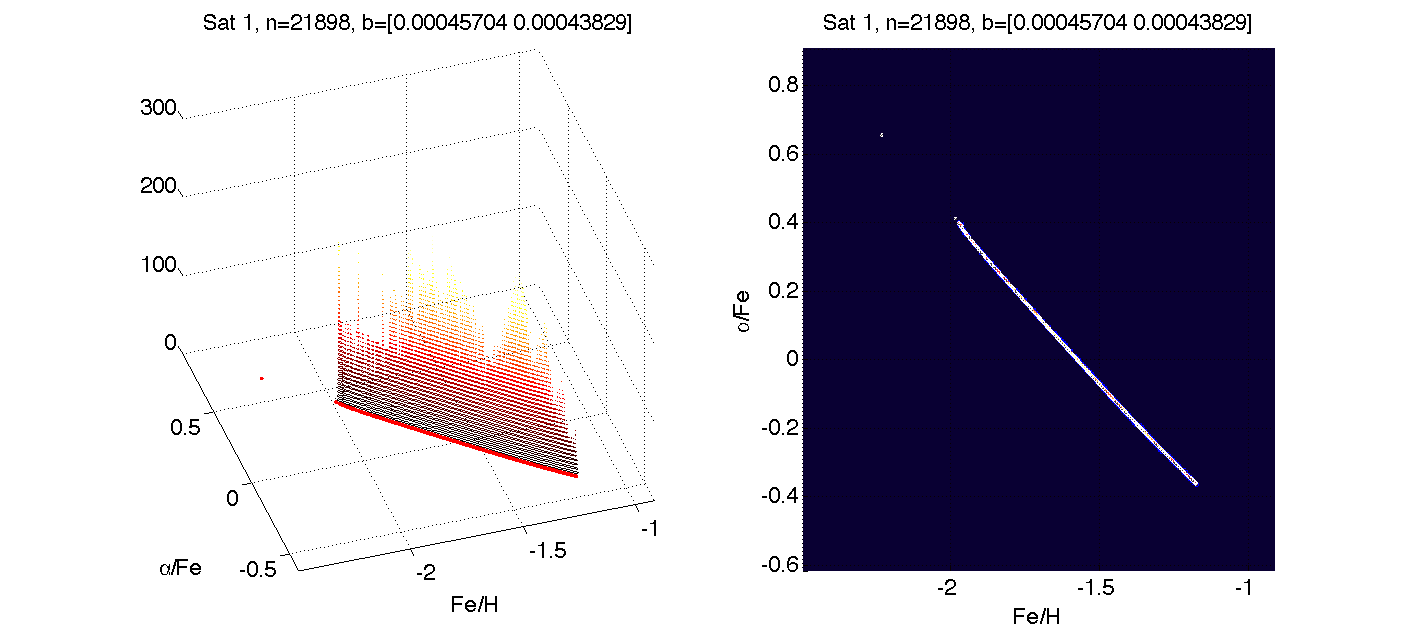
\includegraphics[scale=.5]{wsmooth1_auto_4m.png}
	\end{center}
	\caption{Weighted kernel density estimate for sat 1 with an automatic bandwidth. Approx. 4,000,000 used data points.}
\end{figure}

\begin{figure}
	\begin{center}
		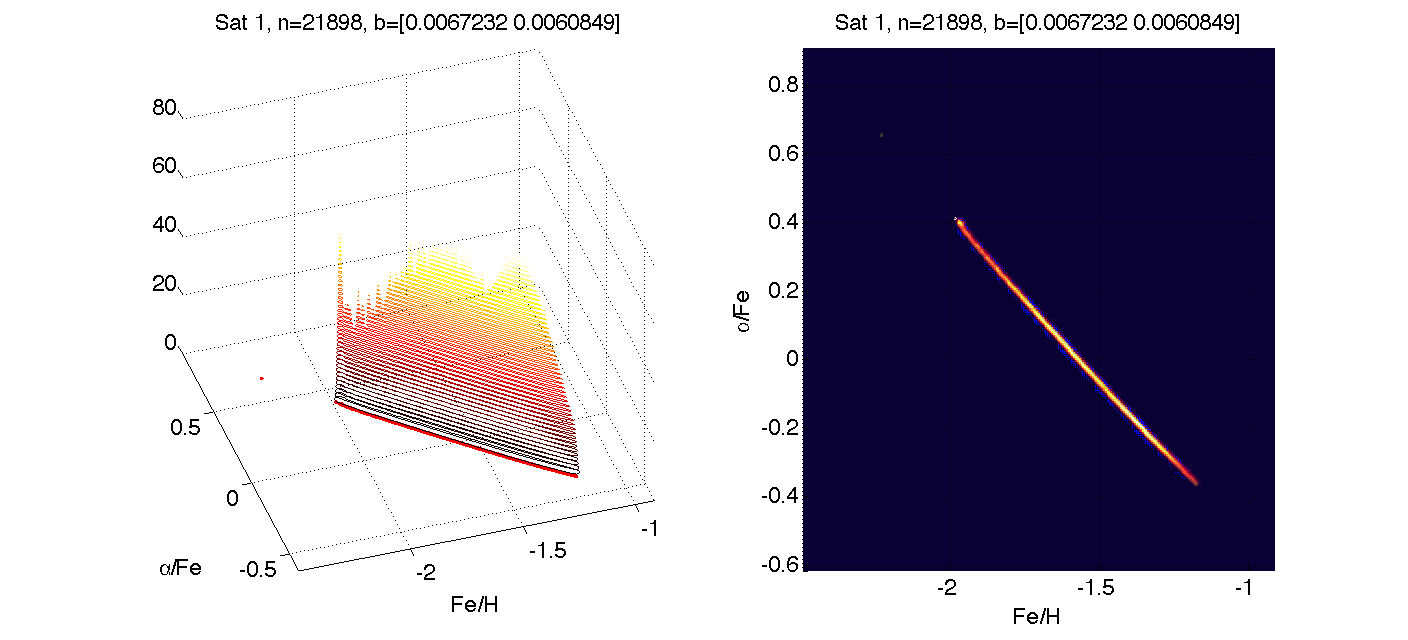
\includegraphics[scale=.5]{wsmooth1_15_4m.png}
	\end{center}
	\caption{Weighted kernel density estimate for sat 1 with a manual bandwidth parameter of 1.5 (via t\_star). Approx. 4,000,000 used data points.}
\end{figure}




\end{document}













